\section{切空间估计}
\label{sec:mrec-tangent}

切空间是流形在一点处的线性近似。第~\ref{chap:manifold-basics}章用曲线的速度或局部坐标定义它，第~\ref{chap:manifold-relations}章说明嵌入子流形的切空间是环境空间的线性子空间。现在只有样本，没有局部坐标，也没有曲线。

本节先说明切空间在什么意义上近似流形，再把这一近似落实为有限样本上的子空间拟合，最后分析拟合误差。局部主成分分析是一种估计方法，它的输出只有在几何近似成立时才是切空间的近似，不能反过来把它当作切空间的定义。

\subsection{切向近似}
\label{sec:mrec-tangent-approx}

在点$\bm p\in M$附近，把环境空间分解为切空间$T=T_{\bm p}M$与它的正交补，即法空间$T^\perp$。把$M$上的点正交投影到$T$，这个映射在$\bm p$处的导数是$T$上的恒等映射，由反函数定理在局部可逆。

它的逆就给出参数化$\bm u\mapsto\bm p+\bm u+g(\bm u)$。也就是说，存在$\bm0$在$T$中的邻域$W$和$C^2$映射$g:W\to T^\perp$，使$M$在$\bm p$附近的部分恰为
\begin{equation}
 \{\bm p+\bm u+g(\bm u):\bm u\in W\},\qquad g(\bm0)=\bm0,\quad Dg(\bm0)=\bm0 .
 \label{eq:mrec-local-graph}
\end{equation}
这里的$g$就是图~\ref{fig:mrec-cylinder}(a)中那些绿色线段的长度和方向：从切平面上的$\bm u$沿法向走$g(\bm u)$，就回到流形。

条件$Dg(\bm0)=\bm0$表达的正是切空间的局部线性作用：沿切向移动$\bm u$，流形在法向上的偏离没有一阶项。对$C^2$的$g$，若它的二阶导数在$W$中某个凸邻域上的范数不超过$K$，由多元Taylor公式，在这个邻域中
\[
 \lVert g(\bm u)\rVert_2\leq\frac K2\lVert\bm u\rVert_2^2 .
\]
多元Taylor展开与余项可参考\BookChapterRef{chap:multivariate-differentiation}{卷二第17章“多元函数微分”}。这个界依赖图函数的坐标，式~\eqref{eq:mrec-reach-normal}给出不依赖坐标的同类界，只用到可达半径。

这是邻域尺度下的近似，不是全局平面表示。以半径为$R$的圆为例，在最低点处取水平切线，图函数是
\[
 g(u)=R-\sqrt{R^2-u^2}=\frac{u^2}{2R}+O(u^4),
\]
二次项正是曲率决定的偏离。但这个表示只在$\lvert u\rvert<R$时有定义，越过左右两端，圆就不再是水平线上的图，切线近似也随之失去意义。

\subsection{局部PCA}
\label{sec:mrec-local-pca}

切向近似说明，在小邻域内，流形上的点主要沿切向展开，法向偏离是二阶小量。于是可以把邻域内的样本当作一团数据，寻找它们展开最多的$m$个方向。这里假定流形的维数$m$已经指定，邻域也已选定，记其中的观测为$\bm x_1,\ldots,\bm x_k$。

\paragraph{局部协方差与主方向}

计算局部质心与局部协方差矩阵
\begin{equation}
 \overline{\bm x}=\frac1k\sum_{j=1}^k\bm x_j,\qquad
 \bm C=\frac1k\sum_{j=1}^k(\bm x_j-\overline{\bm x})(\bm x_j-\overline{\bm x})^\top .
 \label{eq:mrec-local-covariance}
\end{equation}
$\bm C$是$D$阶对称半正定矩阵。取它最大的$m$个特征值对应的标准正交特征向量，排成$\widehat{\bm U}\in\mathbb R^{D\times m}$，其列空间$\widehat S$就是切空间的估计。这一方法称为\term{局部主成分分析}（local principal component analysis）。

主方向的意义来自一个最优性：$\widehat S$在全部$m$维线性子空间中，使中心化样本到子空间的平方距离和最小。记$\bm y_j=\bm x_j-\overline{\bm x}$，取$S$的一组标准正交基排成$\bm V\in\mathbb R^{D\times m}$。$\bm y_j$到$S$的距离的平方，是它的长度平方减去投影长度的平方，所以
\[
 \begin{aligned}
 \sum_j\operatorname{dist}(\bm y_j,S)^2
 &=\sum_j\lVert\bm y_j\rVert_2^2-\sum_j\lVert\bm V^\top\bm y_j\rVert_2^2\\
 &=k\operatorname{tr}\bm C-k\operatorname{tr}(\bm V^\top\bm C\bm V).
 \end{aligned}
\]
第一项与$S$无关，所以最小化距离和等价于最大化$\operatorname{tr}(\bm V^\top\bm C\bm V)$。它的最大值是前$m$个特征值之和，由前$m$个特征向量取到，这一迹极值可参考\BookChapterRef{chap:matrix-approximation}{卷二第15章“矩阵逼近”}。在全部$m$维仿射平面中，到样本的平方距离和最小的是$\overline{\bm x}+\widehat S$。

\paragraph{子空间、基与平面}

这里有三个不同的对象。$\widehat S$是方向子空间，是对$T_{\bm p}M$的估计。$\widehat{\bm U}$只是它的一组标准正交基，右乘任何$m$阶正交矩阵仍是同一个子空间的基，所以比较估计与真值时只能比较子空间，例如用主夹角。$\overline{\bm x}+\widehat S$是拟合平面，它还带有位置信息，而局部质心一般不在流形上，也不等于$\bm p$。

\paragraph{矩阵的秩不是流形的维数}

有限样本的协方差矩阵的秩不能直接当作真实维数。带噪声时$\bm C$一般满秩，秩等于$\min(D,k-1)$，与$m$无关；无噪声时，流形的弯曲也使样本不落在任何$m$维平面上，$\bm C$的秩仍可能大于$m$。

例~\ref{ex:mrec-one-sided}的三个点在一条曲线上，$m=1$，却算出秩为$2$的$\bm C$，两个特征值约为$4.43\times10^{-2}$和$2.0\times10^{-4}$。谱中前$m$个特征值明显大于其余，可以作为维数的线索，但要把它当作判断，就必须结合下一小节的误差分析说明“明显”的界限。本节始终把$m$看作已知。

\subsection{切空间估计的误差}
\label{sec:mrec-tangent-error}

现在估计$\widehat S$偏离$T=T_{\bm p}M$多远。误差有三个来源：流形在邻域内的弯曲，邻域内样本在切向上的分布，以及观测扰动。下面把它们分别写进局部协方差矩阵，再用特征子空间的扰动界控制方向的偏离。

所用的工具是\BookChapterRef{chap:condition-and-spectral-perturbation}{卷二第7章“条件数与谱扰动”}中的Davis--Kahan谱隙界。设对称矩阵$\bm C_0$扰动为$\bm C=\bm C_0+\bm E$，$\gamma=\lambda_m(\bm C_0)-\lambda_{m+1}(\bm C)>0$，则两者的前$m$个特征子空间的最大主夹角$\theta_{\max}$满足
\begin{equation}
 \sin\theta_{\max}\leq\frac{\lVert\bm E\rVert_2}{\gamma}.
 \label{eq:mrec-davis-kahan}
\end{equation}

\paragraph{误差的分解}

设邻域中观测$\bm x_j$对应的真实采样点$\bm p_j$满足$\lVert\bm p_j-\bm p\rVert_2\leq r$。把$\bm p_j-\bm p$分解为切向部分$\bm u_j\in T$与法向部分$\bm n_j\in T^\perp$，在图表示成立的范围内$\bm n_j=g(\bm u_j)$，于是
\[
 \bm x_j=\bm p+\bm u_j+\bm n_j+\bm e_j,\qquad\lVert\bm e_j\rVert_2\leq\sigma .
\]

用上划线表示邻域平均，记
\[
 \bm a_j=\bm u_j-\overline{\bm u}\in T,\qquad
 \bm b_j=(\bm n_j-\overline{\bm n})+(\bm e_j-\overline{\bm e}).
\]
则$\bm x_j-\overline{\bm x}=\bm a_j+\bm b_j$，切向展开全部在$\bm a_j$里，弯曲和噪声全部在$\bm b_j$里。代入式~\eqref{eq:mrec-local-covariance}，
\[
 \bm C=\bm C_0+\bm E,\qquad\bm C_0=\frac1k\sum_j\bm a_j\bm a_j^\top ,
\]
\[
 \bm E=\frac1k\sum_j\bigl(\bm a_j\bm b_j^\top+\bm b_j\bm a_j^\top+\bm b_j\bm b_j^\top\bigr).
\]

$\bm C_0$的像在$T$中，在$T^\perp$上为零。记它在$T$上的最小特征值为$\lambda_T$，它度量样本在最不充分的那个切向上展开了多少，第~\ref{sec:mrec-coverage}节的水平线采样中$\lambda_T=0$。

为了估计$\bm E$，先注意对任意向量组，
\[
 \Bigl\lVert\frac1k\sum_j\bm v_j\bm w_j^\top\Bigr\rVert_2\leq\max_j\lVert\bm v_j\rVert_2\max_j\lVert\bm w_j\rVert_2 .
\]
这是因为对单位向量$\bm y,\bm z$，由Cauchy不等式，$\bm y^\top\bm v_j$与$\bm w_j^\top\bm z$的绝对值分别不超过$\lVert\bm v_j\rVert_2$和$\lVert\bm w_j\rVert_2$，它们的乘积取平均不会变大。

再看两类向量的长度。由$\lVert\bm u_j\rVert_2\leq r$，得$\lVert\bm a_j\rVert_2\leq2r$。由式~\eqref{eq:mrec-reach-normal}，$\lVert\bm n_j\rVert_2\leq r^2/(2\tau)$，所以$\bm b_j$的长度不超过
\begin{equation}
 \beta=\frac{r^2}\tau+2\sigma .
 \label{eq:mrec-beta}
\end{equation}

\begin{theorem}[局部PCA的方向误差]
\label{thm:mrec-local-pca-error}
在上述假设下，$\lVert\bm E\rVert_2\leq4r\beta+\beta^2$，其中$\beta$由式~\eqref{eq:mrec-beta}给出。若$\lambda_T>0$且$4r\beta+\beta^2\leq\lambda_T/2$，则估计子空间$\widehat S$与$T_{\bm p}M$的最大主夹角满足
\begin{equation}
 \sin\theta_{\max}\leq\frac{2(4r\beta+\beta^2)}{\lambda_T}.
 \label{eq:mrec-local-pca-error}
\end{equation}
\end{theorem}
\begin{proof}
由前面的不等式，$\bm E$的三部分分别不超过$2r\beta$、$2r\beta$和$\beta^2$，所以$\lVert\bm E\rVert_2\leq4r\beta+\beta^2$。

$\bm C_0$的前$m$个特征值不小于$\lambda_T$，其余为零，前$m$个特征子空间就是$T$。由Weyl不等式，$\bm C$的第$m+1$个特征值不超过$\lVert\bm E\rVert_2$，于是
\[
 \gamma\geq\lambda_T-\lVert\bm E\rVert_2\geq\frac{\lambda_T}2 .
\]
代入式~\eqref{eq:mrec-davis-kahan}，即得式~\eqref{eq:mrec-local-pca-error}。
\end{proof}

\paragraph{方向覆盖与尺度的权衡}

分母$\lambda_T$要求样本在每个切向上都有展开，这正是第~\ref{sec:mrec-coverage}节所说的方向分布条件。若邻域内的样本在切向上铺得比较均匀，$\lambda_T$与$r^2$同量级，例如在$m$维圆盘上均匀分布时为$r^2/(m+2)$。设$\lambda_T\geq c\,r^2$，忽略高阶项，界的主要部分为
\begin{equation}
 \sin\theta_{\max}\lesssim\frac8c\Bigl(\frac r\tau+\frac{2\sigma}r\Bigr).
 \label{eq:mrec-pca-tradeoff}
\end{equation}
第一项来自弯曲，随$r$增大；第二项来自扰动，随$r$增大而减小。

所以缩小邻域并不总是更好。无噪声时取小的$r$可以压低弯曲误差，但$r$不能小到邻域内样本不足以在各切向上铺开，这要求$r$明显大于覆盖精度。有噪声时两项在$r$约为$\sqrt{2\sigma\tau}$处平衡，再小反而更差。图~\ref{fig:mrec-pca}(c)对单位圆上的单侧邻域算出了实际的方向误差，它在两条虚线相交的量级上取到最小值，曲线形状与式~\eqref{eq:mrec-pca-tradeoff}一致。

这个界是最坏情形的估计，常数偏大。取下面例子中的$c=\tfrac16$，要使定理的条件$4r\beta+\beta^2\leq\lambda_T/2$成立，无噪声时大约要$r\leq\tau/48$。定理的价值在于说明误差怎样依赖$r$、$\tau$、$\sigma$和$\lambda_T$，而不是给出紧的数值。

\begin{example}[单侧邻域的倾斜]
\label{ex:mrec-one-sided}
在抛物线$y=u^2/(2R)$上取$\bm p=(0,0)$，它在原点附近近似半径为$R$的圆，切线为横轴。

若邻域样本对称地取在$u=-h,0,h$处，由对称性，横向与纵向的协方差为零，主方向恰为横轴，横向方差$2h^2/3$远大于纵向方差$h^4/(18R^2)$。

若只取单侧的$u=0,h,2h$，三点的纵坐标是$0,\ h^2/(2R),\ 2h^2/R$，横向均值$\overline u=h$，纵向均值$\overline y=5h^2/(6R)$。逐项计算协方差矩阵的元素，得到
\[
 C_{uu}=\frac{2h^2}3,\qquad C_{uy}=\frac{2h^3}{3R},\qquad C_{yy}=\frac{13h^4}{18R^2}.
\]

主方向与横轴的夹角$\varphi$满足
\[
 \tan2\varphi=\frac{2C_{uy}}{C_{uu}-C_{yy}}\approx\frac{2h}R,
\]
所以$\varphi\approx h/R$。这恰好是抛物线在质心横坐标$u=h$处的切线斜率：估计出的其实是质心附近的切方向，相对于$T_{\bm p}M$的偏离是$r/\tau$量级，与定理中的弯曲项一致。

取$R=1$，$h=0.25$代入，$C_{uu}\approx0.0417$，$C_{uy}\approx0.0104$，$C_{yy}\approx0.0028$，于是$\tan2\varphi\approx0.536$，$\varphi\approx14.1^\circ$，而$\arctan(h/R)\approx14.0^\circ$。
\end{example}

图~\ref{fig:mrec-pca}(a)(b)画出了这两种邻域。对称邻域把弯曲的影响抵消了，单侧邻域则把主方向带向质心处的切线，这一倾斜不会因为增加样本而消失。

\begin{BookInlineFigure}
  \centering
  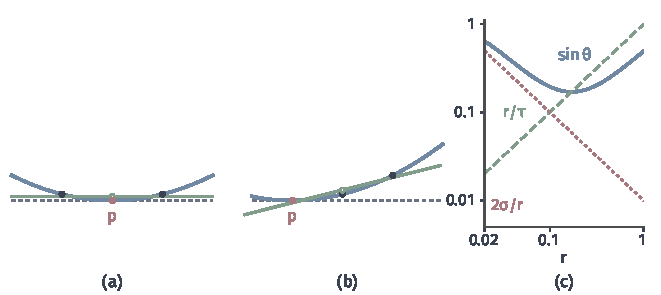
\includegraphics[width=112mm]{figures/04-spaces-measures-and-geometry/04-manifolds/matplotlib/mrec-pca/figure.pdf}
  \caption{局部PCA的方向误差。(a)(b) 抛物线$y=u^2/2$上$h=0.25$的对称与单侧邻域，黑点是样本，空心点是局部质心，绿线是主方向，虚线是$\bm{p}$处的真实切线；单侧时主方向倾斜$14.1^\circ$。(c) 单位圆上单侧弧$[0,r]$内$41$个样本加法向扰动$\sigma=0.005$时的实际误差（蓝），与弯曲项$r/\tau$（绿）、扰动项$2\sigma/r$（红）的比较，纵轴和横轴都取对数。}
  \label{fig:mrec-pca}
\end{BookInlineFigure}
